\documentclass{article}

\usepackage{kyrem1sty}
\usepackage{PRIMEarxiv}
\usepackage{circuitikz}
\usepackage[utf8]{inputenc} % allow utf-8 input
\usepackage[T1]{fontenc}    % use 8-bit T1 fonts
\usepackage{hyperref}       % hyperlinks
\usepackage{url}            % simple URL typesetting
\usepackage{booktabs}       % professional-quality tables
\usepackage{amsfonts}       % blackboard math symbols
\usepackage{nicefrac}       % compact symbols for 1/2, etc.
\usepackage{microtype}      % microtypography
\usepackage{lipsum}
\usepackage{fancyhdr}       % header
\usepackage{graphicx}       % graphics
\graphicspath{{media/}}     % organize your images and other figures under media/ folder
\usepackage{xcolor}
%Header
\pagestyle{fancy}
\thispagestyle{empty}
\rhead{ \textit{ }} 

\hypersetup{%
  colorlinks=true,%
  linkcolor=blue,%
  citecolor=blue,%
  filecolor=blue,%
  menucolor=blue,%
  urlcolor=blue,%
  pdfnewwindow=true,%
  pdfstartview=FitBH
}   
\usetikzlibrary{positioning,chains, fit, arrows.meta}
\usepackage{caption}

% Update your Headers here
\fancyhead[LO]{Stacked Deep-Q Networks for Forex Trading—Harbour \& Olgun}
% \fancyhead[RE]{Firstauthor and Secondauthor} % Firstauthor et al. if more than 2 - must use \documentclass[twoside]{article}


%% Title
\title{Stacked Deep-Q Networks for Forex Trading}

\author{
  James Harbour \\
  Math and CS \\
  University of Virginia \\
  \texttt{gtr8rh@virginia.edu} \\
   \And
  Deniz Olgun \\
  Neuro and CS \\
  University of Virginia \\
  \texttt{epv2kz@virginia.edu} \\
}

\begin{document}
\maketitle

\begin{abstract}
This paper presents an innovative approach to automated trading in the Forex market, leveraging the power of Deep Q-Networks (DQNs) and sentiment analysis to inform trading decisions. Recognizing the Forex market's continuous operation and the abundance of public data it offers, we propose a multi-tiered machine learning strategy aimed at executing profitable trades with minimal exposure to underlying asset price volatility. Our methodology involves the development of three interconnected DQNs: the first processes price time series data to recommend actions (buy, hold, or sell); the second combines price data with sentiment analysis of global news articles to forecast currency pair price movements; and the third synthesizes outputs from the first two networks to finalize trading decisions. This strategy capitalizes on the predictive power of DQNs and the informative value of real-time news sentiment, aiming to achieve non-zero risk-adjusted returns that are uncorrelated with market movements. Preliminary results, drawn from backtesting and anticipated live market trials via the MetaTrader API, suggest a promising avenue for automated Forex trading strategies that enhance profitability while managing risk. This work builds on existing literature by incorporating reinforcement learning into Forex trading and extends previous applications of sentiment analysis in cryptocurrency markets to the realm of fiat currencies.
\end{abstract}


% keywords can be removed
\keywords{Forex \and Deep Q learning \and Sentiment Analysis}


\section{Introduction}
\subsection{Problem Definition}

There is considerable interest in developing automated trading strategies for financial instruments. Foreign currency exchanges (Forex) are one of the most liquid financial markets, trading continuously with high volume for 24 hours 5 days a week. In this setting where vast amounts of public data are available and information asymmetry is low, we anticipate that machine learning strategies would be useful. 

Our input data will be a medium-frequency price time series on currency pairs against USD and global news articles. Our analysis will transform these data to produce a policy decision to buy, hold, or sell each currency pair at the given timepoint. The portfolio of currency pairs will then be hedged against a basket of options that minimizes exposure to the prices of the underlying assets.

\section{Proposed Idea}
For this application project, we plan to explore applications of Deep Q-networks (DQN) in various architectures. We also plan to use a text embedding and sentiment analysis library to classify news articles as an input feature. Our tentative plan is to develop two data pre-processing networks which will feed into a third policy network which will actually perform the trade using a pre-existing API.

\section{Experiment Setup}
 Experiment Setup: describe datasets (forex data), preprocessing (normalization, RNN data / selecting 5 datapoints), hyper-parameters (just implement randomized search), optimization methods (IDEK), different model architectures with varying levels of complexity, 





\subsection{Datasets}

Our experiment utilizes intraday foreign exchange time series data for EUR/USD collected from the Oanda broker via the python package \textit{pyfinancialdata} \cite{williams:20}. We utilize frequencies of both hourly and minute-to-minute. The dataset consists of Open, High, Low, Close values over the time interval.

INCLUDE GRAPH OF FOREX

\subsection{Preprocessing}

For input into the LSTM, following the Box-Jenkins approach to time series modelling we analyzed the partial autocorrelation function for our minute-level time-series to determine the appropriate window size. From figure \ref{fig:pacf}, we chose to use a time lag of $ 5 $. 

INCLUDE PACF FIGURE

We then transformed our time-series to a series of over-lapping subsequences. For example, if we used a time lag of $ 3 $, then we would perform the following transformation:

\[
  [1,2,3,4,5,6,7] \mapsto [1,2,3], [2,3,4], [3,4,5], [4,5,6], [5,6,7]
\]

As financial data has an underlying meaning associated to its magnitude, we felt any normalization to be unwise. As such, we left the time-series largely untouched when feeding into the deep-Q network.


\section{Model Architectures}

The intuition of feeding in a sequence of currency values into a model and predicting, say, the next few values naturally leads one to consider a recurrent neural network (RNN) architecture. These are a class of neural networks specifically designed to handle sequential dataand, unlike traditional feedforward networks, RNNs can capture dynamic temporal behaviors as they have an internal state that serves as a form of memory. In practice, one can treat an RNN as a feedforward neural network with a hidden layer block for each time step. This unravelling intuition can be seen in figure \ref{fig:unravel}.

\begin{figure}[H]
  \centering
  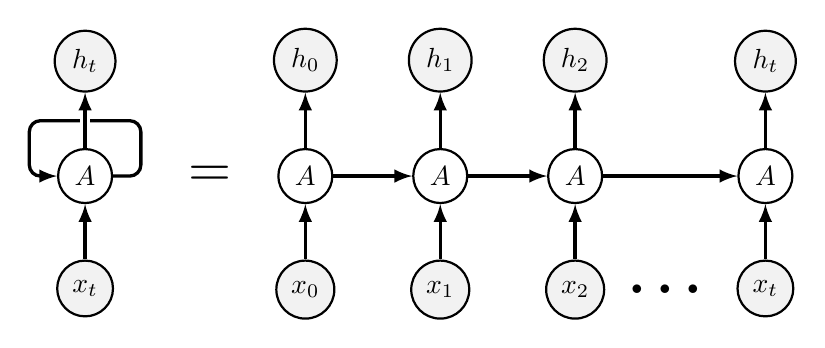
\begin{tikzpicture}[item/.style={circle,draw,thick,align=center},
itemc/.style={item,on chain,join}]
 \begin{scope}[start chain=going right,nodes=itemc,every
 join/.style={-latex,very thick},local bounding box=chain]
 \path node (A0) {$A$} node (A1) {$A$} node (A2) {$A$} node[xshift=2em] (At)
 {$A$};
 \end{scope}
 \node[left=1em of chain,scale=2] (eq) {$=$};
 \node[left=2em of eq,item] (AL) {$A$};
 \path (AL.west) ++ (-1em,2em) coordinate (aux);
 \draw[very thick,-latex,rounded corners] (AL.east) -| ++ (1em,2em) -- (aux) 
 |- (AL.west);
 \foreach \X in {0,1,2,t} 
 {\draw[very thick,-latex] (A\X.north) -- ++ (0,2em)
 node[above,item,fill=gray!10] (h\X) {$h_\X$};
 \draw[very thick,latex-] (A\X.south) -- ++ (0,-2em)
 node[below,item,fill=gray!10] (x\X) {$x_\X$};}
 \draw[white,line width=0.8ex] (AL.north) -- ++ (0,1.9em);
 \draw[very thick,-latex] (AL.north) -- ++ (0,2em)
 node[above,item,fill=gray!10] {$h_t$};
 \draw[very thick,latex-] (AL.south) -- ++ (0,-2em)
 node[below,item,fill=gray!10] {$x_t$};
 \path (x2) -- (xt) node[midway,scale=2,font=\bfseries] {\dots};
\end{tikzpicture}
\caption{Unravelling of a simple recurrent neural network}
\label{fig:unravel}
\end{figure}

Applying backpropogation to this type of time-unfolded feedforward network is known as backpropogation through time (BPTT). One main difficulty that arises from this model when running BPTT is that the multiplicative nature of chain rule leads to exponentially growing or decaying gradients over time, thus presenting a massive barrier to learning long-term dependencies. In working with foreign exchange data over multiple years, this initially somewhat minor problem becomes incredibly pertinent and thus forces us to consider more complicated recurrent architectures.

\subsection{LSTM}
Long Short-Term Memory (LSTM) networks were specifically designed to tackle this gradient decay/explosion by introducing memory cell and gating mechanisms to selectively remember and forget certain data. Intuitively, this selectiveness in memory prevents the content held within the entire network from growing too large as time moves. Mathematically, BPTT applied to this architecture leads to linear combinations of gradients instead of multiplicative combinations, thus explaining why LSTM is an ample drop-in fix over simple RNN. For the reader's edification, we have included a depiction of an LSTM cell below in figure \ref{fig:lstm}     



\begin{figure}[H]

\centering
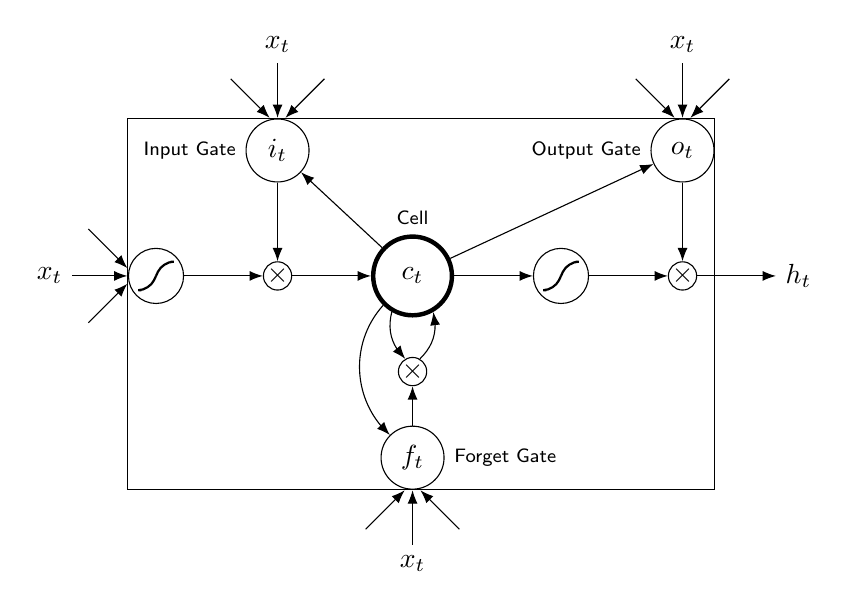
\begin{tikzpicture}[
    prod/.style={circle, draw, inner sep=0pt},
    ct/.style={circle, draw, inner sep=5pt, ultra thick, minimum width=10mm},
    ft/.style={circle, draw, minimum width=8mm, inner sep=1pt},
    filter/.style={circle, draw, minimum width=7mm, inner sep=1pt, path picture={\draw[thick, rounded corners] (path picture bounding box.center)--++(65:2mm)--++(0:1mm);
    \draw[thick, rounded corners] (path picture bounding box.center)--++(245:2mm)--++(180:1mm);}},
    mylabel/.style={font=\scriptsize\sffamily},
    >=LaTeX
    ]

\node[ct, label={[mylabel]Cell}] (ct) {$c_t$};
\node[filter, right=of ct] (int1) {};
\node[prod, right=of int1] (x1) {$\times$}; 
\node[right=of x1] (ht) {$h_t$};
\node[prod, left=of ct] (x2) {$\times$}; 
\node[filter, left=of x2] (int2) {};
\node[prod, below=5mm of ct] (x3) {$\times$}; 
\node[ft, below=5mm of x3, label={[mylabel]right:Forget Gate}] (ft) {$f_t$};
\node[ft, above=of x2, label={[mylabel]left:Input Gate}] (it) {$i_t$};
\node[ft, above=of x1, label={[mylabel]left:Output Gate}] (ot) {$o_t$};

\foreach \i/\j in {int2/x2, x2/ct, ct/int1, int1/x1,
            x1/ht, it/x2, ct/it, ct/ot, ot/x1, ft/x3}
    \draw[->] (\i)--(\j);

\draw[->] (ct) to[bend right=45] (ft);

\draw[->] (ct) to[bend right=30] (x3);
\draw[->] (x3) to[bend right=30] (ct);

\node[fit=(int2) (it) (ot) (ft), draw, inner sep=0pt] (fit) {};

\draw[<-] (fit.west|-int2) coordinate (aux)--++(180:7mm) node[left]{$x_t$};
\draw[<-] ([yshift=1mm]aux)--++(135:7mm);
\draw[<-] ([yshift=-1mm]aux)--++(-135:7mm);

\draw[<-] (fit.north-|it) coordinate (aux)--++(90:7mm) node[above]{$x_t$};
\draw[<-] ([xshift=1mm]aux)--++(45:7mm);
\draw[<-] ([xshift=-1mm]aux)--++(135:7mm);

\draw[<-] (fit.north-|ot) coordinate (aux)--++(90:7mm) node[above]{$x_t$};
\draw[<-] ([xshift=1mm]aux)--++(45:7mm);
\draw[<-] ([xshift=-1mm]aux)--++(135:7mm);

\draw[<-] (fit.south-|ft) coordinate (aux)--++(-90:7mm) node[below]{$x_t$};
\draw[<-] ([xshift=1mm]aux)--++(-45:7mm);
\draw[<-] ([xshift=-1mm]aux)--++(-135:7mm);
\end{tikzpicture}
\caption{LSTM cell}
\label{fig:lstm}
\end{figure}

\subsection{Deep Q-Networks}


One point that is not at all obvious from a time-series point of view is how to make optimal trading decisions based up predictive data. Even with a way to look ahead into the future, one requires the extra input of some type of trading strategy to actually convert this data-edge into genuine profit. This is difficult in practice and the main methods in practice, known as ``technical analysis,'' are seen as financial astrology by many. As such, one way to sidestep this problem is to simply outsource the trading decision making to a learning algorithm. This places us in the setting of reinforcement learning, namely Q-learning.


Q-learning is a fundamental algorithm in reinforcement learning that enables an agent to learn the optimal action to take in a given state. The core concept revolves around the Q-function, denoted as $Q(s, a)$, which estimates the expected total reward an agent can obtain by starting from state $s$, taking action $a$, and following an optimal policy thereafter.

\subsubsection{State and Action Spaces}

To formalize the environment in which the agent operates, we define two key components:
\begin{itemize}
  \item The \textbf{state space}, $\mathcal{S}$, encompasses all possible states the agent can encounter. It can be either discrete or continuous, depending on the nature of the problem.
  \item The \textbf{action space}, $\mathcal{A}$, represents the set of actions available to the agent at each state. Similar to the state space, the action space can be discrete or continuous.
\end{itemize}

\subsubsection{Updating Q-Values: The Bellman Equation}

The Q-values are iteratively updated using the Bellman equation, which forms the foundation of Q-learning:
\begin{equation}
  Q_{\text{new}}(s_t, a_t) = Q(s_t, a_t) + \alpha \left[r_{t+1} + \gamma \max_{a} Q(s_{t+1}, a) - Q(s_t, a_t)\right]
\end{equation}
where $\alpha$ represents the learning rate, controlling the step size of each update, and $\gamma$ is the discount factor that balances the importance of immediate and future rewards. The equation adjusts the Q-value based on the received reward $r_{t+1}$ and the maximum expected future reward from the subsequent state $s_{t+1}$.

\subsubsection{Integrating Deep Learning: Deep Q-Networks (DQNs)}

While traditional Q-learning uses a tabular approach to store Q-values, Deep Q-Networks (DQNs) leverage the power of deep neural networks to approximate the Q-function. This extension enables Q-learning to handle high-dimensional state spaces and overcome the limitations of the tabular method.

\subsubsection{DQN Architecture}

A typical DQN architecture consists of the following components:
\begin{itemize}
  \item \textbf{Input Layer:} Accepts the state representation of the environment as input.
  \item \textbf{Hidden Layers:} Comprise multiple layers that extract relevant features and learn complex representations.
  \item \textbf{Output Layer:} Produces the estimated Q-values for each action in the given state.
\end{itemize}


\begin{figure}[!ht]
\centering
\resizebox{1\textwidth}{!}{%
\begin{circuitikz}
\tikzstyle{every node}=[font=\LARGE]
\draw  (3.75,11.5) ellipse (1.75cm and 3cm) node {\LARGE Input} ;


\draw [->, >=Stealth, dashed] (5.5,13.25) -- (9.25,14.75);
\draw [->, >=Stealth, dashed] (5.75,11.75) -- (9.25,11.75);
\draw [->, >=Stealth, dashed] (5.5,10.25) -- (9,8.75);
\draw [->, >=Stealth, dashed] (5.75,12.25) -- (9.25,14.5);
\draw [->, >=Stealth, dashed] (5.75,11.25) -- (9,9);
\draw [, dashed] (12.5,12) ellipse (2.25cm and 6.75cm) node {\LARGE Hidden} ;
\draw  (18.75,16.5) rectangle  node {\LARGE Output} (23,6.75);
\draw [->, >=Stealth] (23.25,14.75) -- (28,14.75);
\draw [->, >=Stealth] (23.25,13) -- (28,13);
\draw [->, >=Stealth] (23.25,8.5) -- (28,8.5);
\node [font=\LARGE] at (29.75,14.75) {$Q(s,a_1)$};
\node [font=\LARGE] at (29.75,13) {$Q(s,a_2)$};
\node [font=\LARGE] at (29.75,8.5) {$Q(s,a_k)$};
\node [font=\LARGE] at (25.5,10.75) {$\vdots$};
\draw [->, >=Stealth] (-2.25,11.75) -- (1.5,11.75);
\node [font=\LARGE] at (-0.5,12.25) {s};
\draw [->, >=Stealth, dashed] (14.75,15.5) -- (18.25,12);
\draw [->, >=Stealth, dashed] (15,11.75) -- (18,11.75);
\draw [->, >=Stealth, dashed] (14.75,8.75) -- (18.25,11.5);
\draw [->, >=Stealth, dashed] (14.75,8) -- (18,8);
\draw [->, >=Stealth, dashed] (15,16) -- (18,16);
\end{circuitikz}
}%

\label{fig:my_label}
\end{figure}

\subsubsection{Training Procedure}

The training process of a DQN involves the following key steps:
\begin{enumerate}
  \item \textbf{Experience Replay:} The agent's experiences, represented as tuples $e_t = (s_t, a_t, r_{t+1}, s_{t+1})$, are stored in a replay buffer. During training, mini-batches of experiences are randomly sampled from this buffer, promoting stability and reducing correlations between samples.
  \item \textbf{Loss Calculation:} The temporal difference error is used to define the loss function:
  \begin{equation}
    L = \left( r_{t+1} + \gamma \max_{a} Q(s_{t+1}, a; \theta^-) - Q(s_t, a_t; \theta) \right)^2
  \end{equation}
  where $\theta$ represents the parameters of the DQN, and $\theta^-$ denotes the parameters of a separate target network.
  \item \textbf{Target Network Updates:} To stabilize the learning process, the target network parameters $\theta^-$ are periodically updated with the parameters of the main DQN $\theta$. This helps mitigate the issue of moving targets and enhances the stability of the algorithm.
\end{enumerate}

By integrating deep learning with Q-learning, DQNs have achieved remarkable success in various domains, enabling agents to learn complex policies directly from high-dimensional sensory inputs.


\subsection{Hyperparameters and Optimization}




\section{Expected Outcome}
We would like to finish implementing this algorithm about 3 weeks before the final due date. This way, we can go beyond backtesting on historical data and test the model's performance live on real markets. We will route the output of our terminal DQN through the MetaTrader API to execute our trades on either a paper account or real assets. We hope to capture non-zero risk-adjusted returns that are uncorrelated with the underlying market. 

\section{Related Works}

\begin{itemize}
    \item Our initial motivation for this project is the recent paper of Otabek and Choi \cite{otabek:24} which combines deep Q-networks, and sentiment analysis to create a trading strategy for bitcoin. This algorithm improves upon previous systematic bitcoin algorithms mainly due to the sentiment analysis addition, and we suspect that such a strategy can be adapted to the world of fiat currencies.
    \item Ayitey Junior et. al. in \cite{ayitey:23} survey the current literature on the application of deep learning, both standard and reinforcement-based, to foreign exchange markets. From this analysis, we see that the vast majority of machine learning applications to this setting are via standard neural network architectures. Only a small minority (2 as of now) utilize reinforcement learning in any fashion. 
    \item As the first application of RL to the Forex market, Carapuço, Neves, and Horta in \cite{carapuco:18} utilize a pure deep-Q based policy network and obtain quite admirable returns. This provides motivation for further refinement of the method as it performs somewhat well without inital added complexity.
\end{itemize}


\section{Datasets}
\subsection{Financial Datasets}
For access to the Forex market, we utilize the REST API inside of \href{https://metaapi.cloud/docs/client/}{MetaApi} for communicating with the exchange, obtaining both historical and real-time currency data, and executing trades

\subsection{Sentiment Analysis Datasets}
For data input into the predictive DQN (similar to \cite{otabek:24}), we utilize relevant news articles acquired via publicly available new agency APIs (see this \href{https://free-apis.github.io/#/categories/News}{database})

\section{Requirements for Final Report}
\begin{itemize}
    \item Experiment Setup: describe datasets (forex data), preprocessing (normalization, RNN data / selecting 5 datapoints), hyper-parameters (just implement randomized search), optimization methods (IDEK), different model architectures with varying levels of complexity, 
    
    \item Experiment Results: LSTM (sharpe, backtesting graph), DQN (sharpe, backtesting graph), DQN + LSTM (sharpe, backtesting graph)
    \item Results Analysis: Do your results meet your expectations? If the results are expected and good, please identify the important factors that lead to success. Otherwise, please identify the unexpected issues in the proposed ideas
    \item Conclusion: Short bit about things we have learned: can say surprising just how much went into non-ML tasks (setting up environment, finding good data, cleaning it, fitting it into pipeline) than actually implementing and testing models. Though we expected that to take some time, it was roughly 90/10. We found python to be an unforgiving language for large projects and that the lack of compile-time type checking together with often cryptic error messages difficult. Setting up ML dashboards to compare model was hard, we were often confused about whether our implementations were actually using the GPU or a single thread, . We were tempted to make our own financial backtesting networks and subsequently found 
\end{itemize}

%Bibliography
\bibliographystyle{unsrt}  
\bibliography{references}  


\end{document}

